\documentclass{article}

\usepackage{graphicx}
\usepackage{tikz}
\usepackage{tikzsymbols}
\usetikzlibrary{calc,patterns,shapes.geometric}
\pagestyle{empty}
\usepackage[margin=0pt]{geometry}
\geometry{papersize={14in,12in}}

\def\centerarc[#1](#2)(#3:#4:#5){\draw[#1] ($(#2)+({#5*cos(#3)},{#5*sin(#3)})$) arc (#3:#4:#5);}

\begin{document}
	\begin{figure}
		\centering
		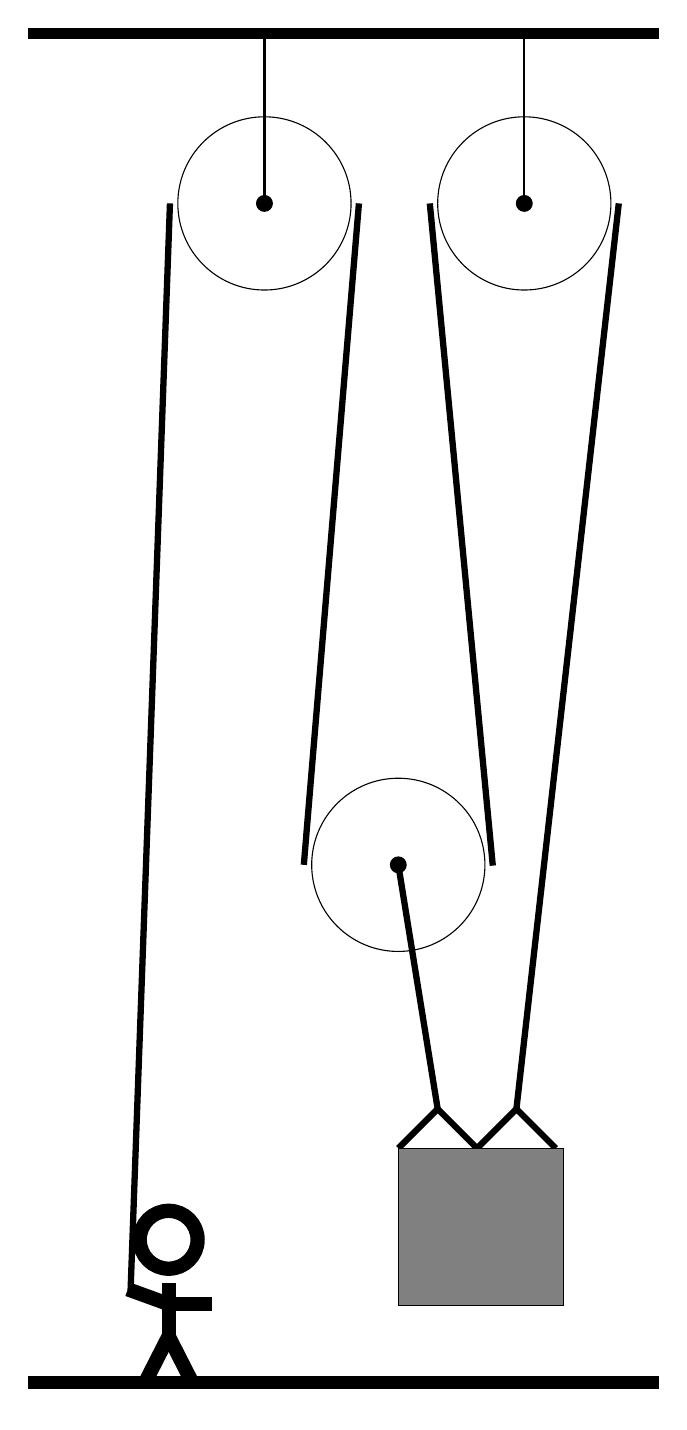
\begin{tikzpicture}
			%%%%% START %%%%%
			\draw[fill=black] (-2, 14) rectangle (6, 14.125);
			
			\draw (1, 11.9) circle (1.1);
			\draw[fill=black] (1, 11.9) circle (0.1);
			\draw[thick] (1, 11.9) -- (1, 14);
			
			\draw (4.3, 11.9) circle (1.1);
			\draw[fill=black] (4.3, 11.9) circle (0.1);
			\draw[thick] (4.3, 11.9) -- (4.3, 14);
			
			\draw (2.7, 3.5) circle (1.1);
			\draw[fill=black] (2.7, 3.5) circle (0.1);
			
			\draw[line width=0.8mm]  (2.7, -0.1) -- (3.2, 0.4) -- (3.7, -0.1) -- (4.2, 0.4) -- (4.7, -0.1);
			\draw[fill=black!50] (2.7, -0.1) rectangle (4.8, -2.1);
			
			\draw[line width=0.8mm](-0.7, -1.9) -- (-0.2, 11.9);
			\centerarc[line width=0.8mm](1, 11.9)(0:180:1.2000000000000002);
			\draw[line width=0.8mm](2.2, 11.9) -- (1.5, 3.5);
			\centerarc[line width=0.8mm](2.7, 3.5)(180:370:1.2000000000000002);
			\draw[line width=0.8mm] (3.9, 3.49) -- (3.1, 11.9);
			\centerarc[line width=0.8mm](4.3, 11.9)(0:180:1.2000000000000002);
			\draw[line width=0.8mm](4.2, 0.4) -- (5.5, 11.9);
			\draw[line width=0.8mm] (3.2, 0.4) -- (2.7, 3.5);
			
			\node at (-0.2, -2) {\Strichmaxerl[10][-20][0]};
			
			\draw[fill=black] (-2, -3) rectangle (6, -3.15);
			%%%%% END %%%%%
		\end{tikzpicture}
	\end{figure}	
\end{document}